\section*{Week 5: Acquisitions / Financial Investments}

\subsection*{Acquisitions and goodwill}


Steps for \textit{allocating the purchase price} :
\begin{enumerate}[noitemsep,topsep=0pt]
	\item Fair value of tangigle assets and liabilities.
	\item \textit{Identifiable} intangile assets: customer relationships, trade names, patents, etc. Subject to amortization with zero salvage value.
	\item Goodwill.  An intangible assets that is not separately identifiable: Everything else (the plug).
\end{enumerate}

\subsection*{Investments}

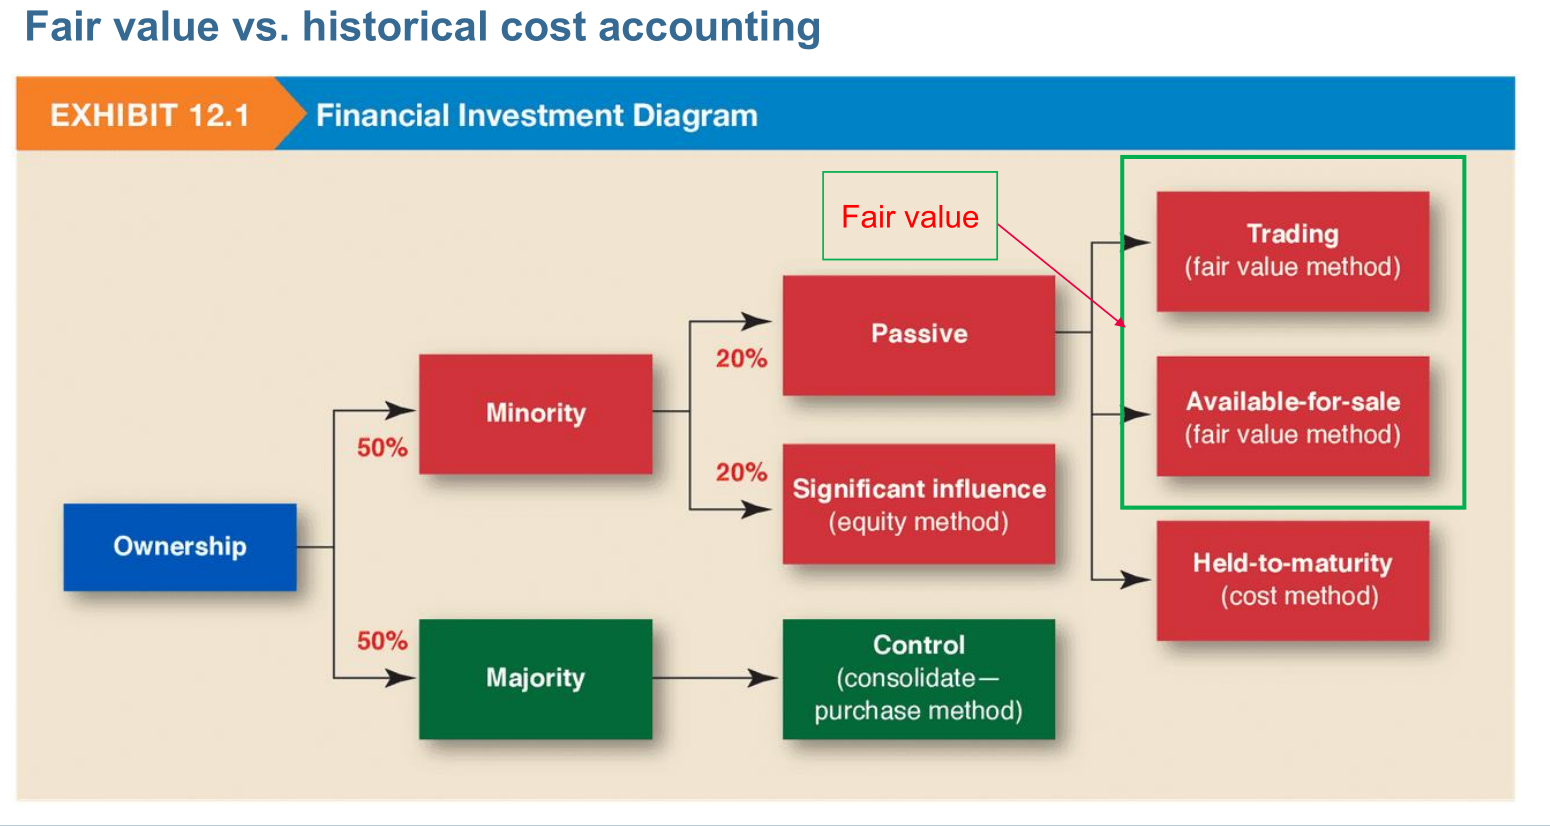
\includegraphics[width=7cm]{assets/fair_value_vs_historical_acct}

\subsection*{Equity Method}

\begin{itemize}[noitemsep,topsep=0pt]
	\item Initially record the investment at acquisition cost.
	\item Adjust the book value of the investment by the investor’s share of dividends and
	earnings or losses.
	\item Record investor’s share of investee’s profit on the investor’s income statements.
	\item Dividends received reduce investment; they do not give rise to dividend income.
\end{itemize}

Example: On 1/1/2010, Zsa Zsa purchased 1,000 shares of Zoltan common stock for \$15
cash per share. This 1,000 shares represents a 30\% interest in Zoltan.
\begin{itemize}[noitemsep,topsep=0pt]
\item Zoltan’s book value per share is \$10. Zsa Zsa is paying a premium because it believes
that Zoltan has unrecorded patents (with a life of 10 years) of \$5 per share.
\item On 6/30, Zsa Zsa received a dividend of \$1 per share on Zoltan common stock.
\item At 12/31/2010 the market price of Zoltan common stock is \$13 per share. (this creates no entry)
\item Zoltan reports its earnings for 2010 as \$20,000.
\item On 12/31/2010 Zsa Zsa amortizes the unrecorded patents (with a life of 10 years) of \$5 per share.
\item on 6/30/2011 Zsa Zsa sells the 1,000 shares of Zoltan common stock for \$17 per share

\end{itemize} 

\newpage

	\begin{tabular}{ |c|c|c||c||c| } 
		\hline
		Dt &  Cash & Inv & RE & Event	 \\ 
		\hline
		1/1   & -15000 & 15000 & & buy@15\\
		6/30  & 1000    & -1000 & & dividend \\
		12/31 &         & 6000  & 6000 & $.3 \cdot 20000$\\ 
		12/31 &         & -500  & -500 & $\frac{5}{10}  1000$ \\    
		6/30 &   17000      & -19500  & -2500 & sell@17 \\      	
		\hline
	\end{tabular}



\subsection*{Passive Investments}

HTM: Hold to maturity \\
AFS: Available for sale \\
TRD: Trading \\

	\begin{tabular}{ |c|c|c| } 
		\hline
			  & B/S Effect & I/S Effect \\ 
		\hline
		HTM (debt) & no &  \\ 
		AFS (debt \& equity) & yes & no \\ 
		TRD (debt \& equity) & yes & yes \\ 
		\hline
	\end{tabular}

Changes in market value affect the balance sheet for AFS and TRD securities. Changes in market value affect income statement only for TRD securiteis.

\subsection*{Take Away}
\begin{itemize}[noitemsep,topsep=0pt]
	\item Passive investments  $\implies$ mark-to-market
	\item With some but not complete control  $\implies$ equity method
	\item Greater than 50\%  ownership $\implies$ consolidate
	\item Whether it is equity or consolidated method makes a big difference on the appearance
	of the statements. Financial ratios (leverage ratios) will be very different
\end{itemize}
